\chapter{Аналитический раздел}
\label{cha:analysis}
%
% % В начале раздела  можно напомнить его цель
%
В соответствии с заданием на курсовой проект необходимо разработать программное
обеспечение, фиксирующее события в системе, инициирующиеся средством ввода информации –
клавиатурой. Так же эту информацию необходимо передавать на удаленный компьютер.
Клавиатура формирует события нажатия кнопок.
Программное обеспечение должно обеспечивать перехват всех действий клавиатуры и
фиксировать эту информацию в файле, для того, чтобы в дальнейшем было возможно произвести
анализ этой информации. 


% Обратите внимание, что включается не ../dia/..., а inc/dia/...
% В Makefile есть соответствующее правило для inc/dia/*.pdf, которое
% берет исходные файлы из ../dia в этом случае.



\section{Анализ подходов реализации}

\begin{itemize}
	\item чтение информации из системного файла устройства “/dev/input/event*”
	\item перехват сообщений клавиатуры в пространстве ядра.
	\end{itemize}
Чтение файла “/dev/input/event*” возможно реализовать в пространстве пользователя. Второй вариант подразумевает под собой написание модуля ядра.
Также перехват сообщений в модуле предоставляет более низкоуровневый доступ к данным,
приходящим от клавиатуры. Именно поэтому предпочтение отдается второму варианту. 

\section{Загружаемые модули ядра Linux }
Ядро Linux относится к категории так называемых монолитных – это означает, что большая часть функциональности операционной системы называется ядром и запускается в привилегированном режиме. Этот подход отличен от подхода микроядра, когда в режиме ядра выполняется только основная функциональность (взаимодействие между процессами [inter-process communication, IPC], диспетчеризация, базовый ввод-вывод [I/O], управление памятью), а остальная функциональность вытесняется за пределы привилегированной зоны (драйверы, сетевой стек, файловые системы). Можно было бы подумать, что ядро Linux очень статично, но на самом деле все как раз наоборот.
Ядро Linux динамически изменяемое – это означает, что вы можете загружать в ядро дополнительную функциональность, выгружать функции из ядра и даже добавлять новые модули, использующие другие модули ядра. Преимущество загружаемых модулей заключается в возможности сократить расход памяти для ядра, загружая только необходимые модули (это может оказаться важным для встроенных систем) \cite{book4}

Linux – не единственное (и не первое) динамически изменяемое монолитное ядро. Загружаемые модули поддерживаются в BSD-системах, Sun Solaris, в ядрах более старых операционных систем, таких как OpenVMS, а также в других популярных ОС, таких как Microsoft Windows и Apple Mac OS X.
\subsection{Устройство модуля ядра}
Загружаемые модули ядра имеют ряд фундаментальных отличий от элементов, интегрированных непосредственно в ядро, а также от обычных программ. Обычная программа содержит главную процедуру (main)в отличие от загружаемого модуля, содержащего функции входа и выхода (в версии 2.6 эти функции можно именовать как угодно). Функция входа вызывается, когда модуль загружается в ядро, а функция выхода – соответственно при выгрузке из ядра. Поскольку функции входа и выхода являются пользовательскими, для указания назначения этих функций используются макросы module\_init и module\_exit . Загружаемый модуль содержит также набор обязательных и дополнительных макросов. Они определяют тип лицензии, автора и описание модуля, а также другие параметры. Пример очень простого загружаемого модуля приведен на рисунке  \ref{fig:an01} .
\begin{figure}[h!]
	\centering
	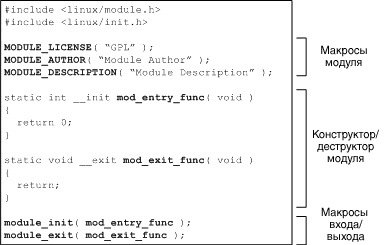
\includegraphics[width=0.6\textwidth]{img/1.png}
	\caption{Пример загружаемого модуля с разделами ELF}
	\label{fig:an01}
\end{figure}
\subsection{Объектный код модуля ядра}
Загружаемый модуль представляет собой просто специальный объектный файл в формате ELF (Executable and Linkable Format). Обычно объектные файлы обрабатываются компоновщиком, который разрешает символы и формирует исполняемый файл. Однако в связи с тем, что загружаемый модуль не может разрешить символы до загрузки в ядро, он остается ELF-объектом. Для работы с загружаемыми модулями можно использовать стандартные средства работы с объектными файлами (которые в версии 2.6 имеют суффикс .ko, от kernel object). Например, если вывести информацию о модуле утилитой objdump, вы обнаружите несколько привычных разделов, в том числе .text (инструкции), .data (инициализированные данные) и .bss (Block Started Symbol или неинициализированные данные)\cite{book4}

В модуле также обнаружатся дополнительные разделы, ответственные за поддержку его динамического поведения. Раздел .init.text содержит код module\_init, а раздел .exit.text – код module\_exit code (рисунок  \ref{fig:an02}). Раздел .modinfo содержит тексты макросов, указывающие тип лицензии, автора, описание и т.д.
\begin{figure}[h!]
	\centering
	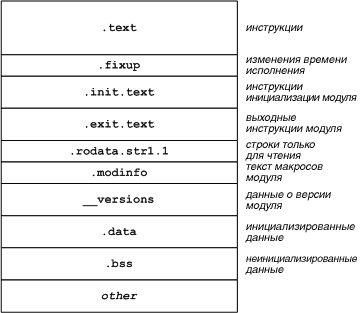
\includegraphics[width=0.6\textwidth]{img/2.png}
	\caption{Пример загружаемого модуля с разделами ELF}
	\label{fig:an02}
\end{figure}
\subsection{Жизненный цикл загружаемого модуля ядра}
Процесс загрузки модуля начинается в пользовательском пространстве с команды insmod (вставить модуль). Команда insmod определяет модуль для загрузки и выполняет системный вызов уровня пользователя init\_module для начала процесса загрузки. Команда insmod для ядра версии 2.6 стала чрезвычайно простой (70 строк кода) за счет переноса части работы в ядро. Команда insmod не выполняет никаких действий по разрешению символов (вместе с командой kerneld), а просто копирует двоичный код модуля в ядро при помощи функции init\_module; остальное делает само ядро.

Функция init\_module работает на уровне системных вызовов и вызывает функцию ядра sys\_init\_module (рисунок  \ref{fig:an03}). Это основная функция для загрузки модуля, обращающаяся к нескольким другим функциям для решения специальных задач. Аналогичным образом команда rmmod выполняет системный вызов функции delete\_module, которая обращается в ядро с вызовом sys\_delete\_module для удаления модуля из ядра.
\begin{figure}[h!]
	\centering
	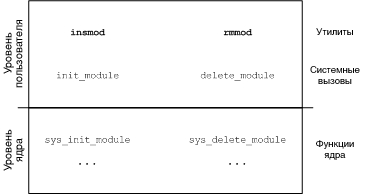
\includegraphics[width=0.6\textwidth]{img/3.png}
	\caption{ Основные команды и функции, участвующие в загрузке и выгрузке модуля}
	\label{fig:an03}
\end{figure}
\subsection{Подробности загрузки модуля}
Теперь давайте взглянем на внутренние функции для загрузки модуля (рисунок \ref{fig:an04}). При вызове функции ядра sys\_init\_module сначала выполняется проверка того, имеет ли вызывающий соответствующие разрешения (при помощи функции capable). Затем вызывается функция load\_module, которая выполняет механическую работу по размещению модуля в ядре и производит необходимые операции (я вскоре расскажу об этом). Функция load\_module возвращает ссылку, которая указывает на только что загруженный модуль. Затем он вносится в двусвязный список всех модулей в системе, и все потоки, ожидающие изменения состояния модуля, уведомляются при помощи специального списка. В конце вызывается функция init() и статус модуля обновляется, чтобы указать, что он загружен и доступен.
\begin{figure}[h!]
	\centering
	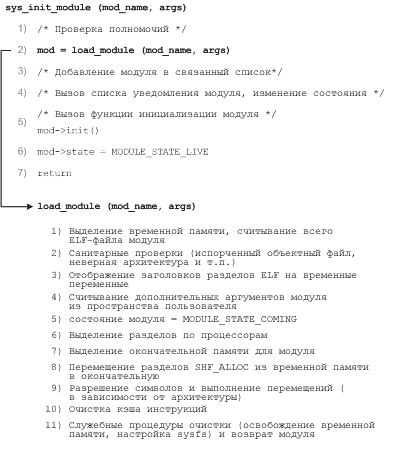
\includegraphics[width=0.6\textwidth]{img/4.png}
	\caption{ Внутренний процесс загрузки модуля(в упрощенном виде)}
	\label{fig:an04}
\end{figure}
Внутренние процессы загрузки модуля представляют собой анализ и управление модулями ELF. Функция load\_module (которая находится в ./linux/kernel/module.c) начинает с выделения блока временной памяти для хранения всего модуля ELF. Затем модуль ELF считывается из пользовательского пространства во временную память при помощи copy\_from\_user. Являясь объектом ELF, этот файл имеет очень специфичную структуру, которая легко поддается анализу и проверке.

Следующим шагом является ряд "санитарных проверок" загруженного образа (является ли ELF-файл допустимым? соответствует ли он текущей архитектуре? и так далее). После того как проверка пройдена, образ ELF анализируется и создается набор вспомогательных переменных для заголовка каждого раздела, чтобы облегчить дальнейший доступ к ним. Поскольку базовый адрес объектного файла ELF равен 0 (до перемещения), эти переменные включают соответствующие смещения в блок временной памяти. Во время создания вспомогательных переменных также проверяются заголовки разделов ELF, чтобы убедиться, что загружаемый модуль корректен.

Дополнительные параметры модуля, если они есть, загружаются из пользовательского пространства в другой выделенный блок памяти ядра (шаг 4), и статус модуля обновляется, чтобы обозначить, что он загружен (MODULE\_STATE\_COMING). Если необходимы данные для процессоров (согласно результатам проверки заголовков разделов), для них выделяется отдельный блок.

В предыдущих шагах разделы модуля загружались в память ядра (временную), и было известно, какие из них используются постоянно, а какие могут быть удалены. На следующем шаге (7) для модуля в памяти выделяется окончательное расположение, и в него перемещаются необходимые разделы (обозначенные в заголовках SHF\_ALLOC или расположенные в памяти во время выполнения). Затем производится дополнительное выделение памяти размера, необходимого для требуемых разделов модуля. Производится проход по всем разделам во временном блоке ELF,, и те из них, которые необходимы для выполнения, копируются в новый блок. Затем следуют некоторые служебные процедуры. Также происходит разрешение символов, как расположенных в ядре (включенных в образ ядра при компиляции), так и временных (экспортированных из других модулей).

Затем производится проход по оставшимся разделам и выполняются перемещения. Этот шаг зависит от архитектуры и соответственно основывается на вспомогательных функциях, определенных для данной архитектуры (./linux/arch/<arch>/kernel/module.c). В конце очищается кэш инструкций (поскольку использовались временные разделы .text), выполняется еще несколько служебных процедур (очистка памяти временного модуля, настройка sysfs) и, в итоге, модуль возвращает load\_module
\subsection{Подробности выгрузки модуля}

Выгрузка модуля фактически представляет собой зеркальное отражение процесса загрузки за исключением того, что для безопасного удаления модуля необходимо выполнить несколько "санитарных проверок". Выгрузка модуля начинается в пользовательском пространстве с выполнения команды rmmod (удалить модуль). Внутри команды rmmod выполняется системный вызов delete\_module, который в конечном счете инициирует sys\_delete\_module внутри ядра (см рисунок \ref{fig:an03} ). Основные операции удаления модуля показаны на рисунке  \ref{fig:an05}.
\begin{figure}[h!]
	\centering
	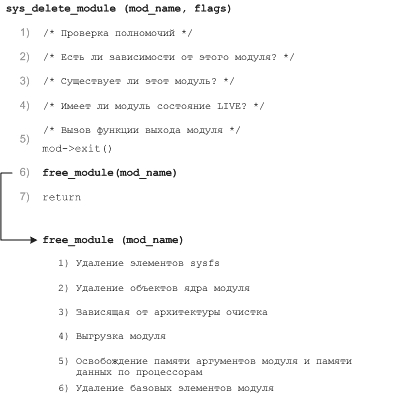
\includegraphics[width=0.6\textwidth]{img/5.png}
	\caption{  Внутренний процесс выгрузки модуля(в упрощенном виде)}
	\label{fig:an05}
\end{figure}
При вызове функции ядра sys\_delete\_module (с именем удаляемого модуля в качестве параметра) сначала выполняется проверка того, имеет ли вызывающий соответствующие разрешения. Затем по списку проверяются зависимости других модулей от данного модуля. При этом используется список modules\_which\_use\_me, содержащий по элементу для каждого зависимого модуля. Если список пуст, т.е. зависимостей не обнаружено, то модуль становится кандидатом на удаление (иначе возвращается ошибка). Затем проверяется, загружен ли модуль. Ничто не запрещает пользователю запустить команду rmmod для модуля, который в данный момент устанавливается, поэтому данная процедура проверяет, активен ли модуль. После нескольких дополнительных служебных проверок предпоследним шагом вызывается функция выхода данного модуля (предоставляемая самим модулем). В заключение вызывается функция free\_module.

К моменту вызова free\_module уже известно, что модуль может быть безопасно удален. Зависимостей не обнаружено, и для данного модуля можно начать процесс очистки ядра. Этот процесс начинается с удаления модуля из различных списков, в которые он был помещен во время установки (sysfs, список модулей и т.д.). Потом инициируется команда очистки, зависящая от архитектуры (она расположена в ./linux/arch/<arch>/kernel/module.c). Затем обрабатываются зависимые модули, и данный модуль удаляется из их списков. В конце, когда с точки зрения ядра очистка завершена, освобождаются различные области памяти, выделенные для модуля, в том числе память для параметров, память для данных по процессорам и память модуля ELF (core и init).
\section{Уведомления в ядре Linux}

\subsection{Уведомители}
Ядро Linux содержит механизм, называемый "уведомителями"(notifiers) или "цепочками уведомлений"(notifiers chains), который позволяет коду ядра просить, чтобы ему сказали, когда что-то интересующее его происходит. Цепочки уведомлений в настоящее время активно используется в ядре; существуют цепочки для событий hotplug памяти, изменения политики частоты процессора, события USB hotplug, загрузка и выгрузка модулей, перезагрузки системы, изменения сетевых устройств и т. д. \cite{book1}

Интерфейс имеет следующий вид:
 \begin{lstlisting}[style=pseudocode,,escapeinside={(@}{@)},caption={struct notifier\_block}] 
 struct notifier_block {
 int (*notifier_call)(struct notifier_block *self,unsigned long event, void *data);	
 struct notifier_block *next;
 int priority;
 };
 \end{lstlisting}
 Таким образом, цепочка уведомлений представляет собой простой, односвязный список без отдельной головы. Подсистема ядра, которая хочет быть уведомленной о конкретных событиях, заполняет структуру notifier\_block и передает ее в:
 
\textit{ int notifier\_chain\_register(struct notifier\_block **chain, 
 struct notifier\_block *notifier);}

Цепочка сохраняется в порядке возрастания приоритета. Отправка события - это вызов:

   \textit{ int notifier\_call\_chain(struct notifier\_block **chain, 
    unsigned long event, void *data);}

Уведомители, зарегистрированные в цепочке, будут вызываться в порядке возрастания приоритета с данными события и данными. Любой уведомитель может вернуть значение с установленным битом NOTIFY\_STOP\_MASK, в результате чего дальнейшие уведомления не будут вызываться. Возвращаемое значение из последнего уведомителя - это возврат из notify\_call\_chain (). В некоторых случаях комбинация NOTIFY\_STOP\_MASK и возвращаемого значения используется, чтобы позволить уведомителям наложить вето на предлагаемые действия. Внутри цепочки уведомлений содержится семафор, который обеспечивает необходимые блокировки.
\subsection{Уведомитель нажатия клавиши}
Существует уведомитель, позволяеющий отслеживать нажатия клавиши:

\textit{int register\_keyboard\_notifier(struct notifier\_block *nb);}

В первый параметр  структуры, передаваемой в функцию,  записываем функцию обратного вызова(callback) для обработки нажатий клавиш клавиатуры.


\subsection{Функция обратного вызова для register\_keyboard\_notifier}
Прототип функции обратного вызова имеет следующий вид:

\textit{int keysniffer\_cb(struct notifier\_block* nblock,
unsigned long code,
void* \_param)
}

\textit{nblock} - указатель на структуру, содержащую эту функцию

\textit{code} - код клавиши клавиатуры

\textit{\_param} - указатель на структуру, описывающую параметры нажатия

Структура, описывающая параметры нажатия, имеет следующий вид:
 \begin{lstlisting}[style=pseudocode,caption={ struct keyboard\_notifier\_param}] 
struct keyboard_notifier_param {
struct vc_data *vc;	
int down;	
int shift;	
unsigned int value;	
};
 \end{lstlisting}
 
\textit{vc\_data} - структура VC для данного события клавиатуры\cite{book2}

 \textit{down} равен 1 когда клавиша нажата, 0 когда клавиша отпущена.

\textit{shift} битовая маска модификации.

\textit{value} - численное значение нажатой клавиши.




\subsection{Хранение информации о нажатых клавишах}
Нажатие клавиш человеком происходит очень быстро, некоторые люди печатают более чем по 300 символов в минуту. Поэтому для логирования этих символов необходима легковесная ram-bases файловая система.  Для целей дебага и логирования в ядро Linux в версии 2.6.11 была введена файловая система debugfs. debugfs - простая в использовании RAM-файловая система. Она существует как простой способ для разработчиков ядра сделать информацию доступной для пользовательского пространства.В отличие от /proc, которая предназначена только для информации о процессе или sysfs, которая имеет строгие правила one-value-per-file, debugfs вообще не имеет правил. Разработчики могут размещать любую информацию, которую они хотят.

Некоторые функции работы с файловой системой debugfs:
\begin{itemize}
	\item Создание каталога:
	
	\textit{struct dentry *debugfs\_create\_dir(const char *name, struct dentry *parent)}

	
	\textit{name} - указатель на строку, содержащую имя создаваемого каталога.
	
	\textit{parent} - указатель на родительский каталог для этого файла. Это должно быть каталог dentry, если параметр установлен. Если этот параметр равен NULL,то каталог будет создан в корне файловой системы debugfs.
	\item Создание файла:
	
	\textit{ struct dentry *debugfs\_create\_file(const char *name, umode\_t mode,
	struct dentry *parent, void *data,
	const struct file\_operations *fops)}

	\textit{name} - указатель на строку, содержащую имя создаваемого каталога.
	
	\textit{mode} - права, которые должен иметь файл.
	
	\textit{parent} - указатель на родительский каталог для этого файла. Это должно быть каталог dentry, если параметр установлен. Если этот параметр равен NULL,то каталог будет создан в корне файловой системы debugfs.
	
	\textit{data} -  указатель на то, что вызывающий хочет получить позже. Указатель inode.i\_private  будет указывает на это значение при  вызове open().
	
	\textit{fops} - указатель на структуру file\_operations, которая должна использоваться для этого файла
	
	\item{Рекурсивное удаление директорий:}
	
	\textit{void debugfs\_remove\_recursive(struct dentry *dentry)}
	
	\textit{dentry} - указатель на удаляемую директорию.
	
	Эта функция рекурсивно удаляет дерево каталогов в debugfs, которое
	 ранее было создана с вызовом другой функции debugfs.Функцию требуется вызывать для удаления в конце работы загружамоего модуля, автоматическая очистка файлов не будет происходить, когда модуль  будет удален.
	

\end{itemize}




%%% Local Variables:
%%% mode: latex
%%% TeX-master: "rpz"
%%% End:
